
%% bare_conf.tex
%% V1.3
%% 2007/01/11
%% by Michael Shell

%% http://www.michaelshell.org/
%% for current contact information.
%%
%% This is a skeleton file demonstrating the use of IEEEtran.cls
%% (requires IEEEtran.cls version 1.7 or later) with an IEEE conference paper.
%%
%% Support sites:
%% http://www.michaelshell.org/tex/ieeetran/
%% http://www.ctan.org/tex-archive/macros/latex/contrib/IEEEtran/
%% and
%% http://www.ieee.org/

%%*************************************************************************
%% Legal Notice:
%% This code is offered as-is without any warranty either expressed or
%% implied; without even the implied warranty of MERCHANTABILITY or
%% FITNESS FOR A PARTICULAR PURPOSE! 
%% User assumes all risk.
%% In no event shall IEEE or any contributor to this code be liable for
%% any damages or losses, including, but not limited to, incidental,
%% consequential, or any other damages, resulting from the use or misuse
%% of any information contained here.
%%
%% All comments are the opinions of their respective authors and are not
%% necessarily endorsed by the IEEE.
%%
%% This work is distributed under the LaTeX Project Public License (LPPL)
%% ( http://www.latex-project.org/ ) version 1.3, and may be freely used,
%% distributed and modified. A copy of the LPPL, version 1.3, is included
%% in the base LaTeX documentation of all distributions of LaTeX released
%% 2003/12/01 or later.
%% Retain all contribution notices and credits.
%% ** Modified files should be clearly indicated as such, including  **
%% ** renaming them and changing author support contact information. **
%%
%% File list of work: IEEEtran.cls, IEEEtran_HOWTO.pdf, bare_adv.tex,
%%                    bare_conf.tex, bare_jrnl.tex, bare_jrnl_compsoc.tex
%%*************************************************************************

% *** Authors should verify (and, if needed, correct) their LaTeX system  ***
% *** with the testflow diagnostic prior to trusting their LaTeX platform ***
% *** with production work. IEEE's font choices can trigger bugs that do  ***
% *** not appear when using other class files.                            ***
% The testflow support page is at:
% http://www.michaelshell.org/tex/testflow/



% Note that the a4paper option is mainly intended so that authors in
% countries using A4 can easily print to A4 and see how their papers will
% look in print - the typesetting of the document will not typically be
% affected with changes in paper size (but the bottom and side margins will).
% Use the testflow package mentioned above to verify correct handling of
% both paper sizes by the user's LaTeX system.
%
% Also note that the "draftcls" or "draftclsnofoot", not "draft", option
% should be used if it is desired that the figures are to be displayed in
% draft mode.
%
\documentclass[conference]{IEEEtran}
\usepackage{blindtext, graphicx, subfigure}
% Add the compsoc option for Computer Society conferences.
%
% If IEEEtran.cls has not been installed into the LaTeX system files,
% manually specify the path to it like:
% \documentclass[conference]{../sty/IEEEtran}





% Some very useful LaTeX packages include:
% (uncomment the ones you want to load)


% *** MISC UTILITY PACKAGES ***
%
%\usepackage{ifpdf}
% Heiko Oberdiek's ifpdf.sty is very useful if you need conditional
% compilation based on whether the output is pdf or dvi.
% usage:
% \ifpdf
%   % pdf code
% \else
%   % dvi code
% \fi
% The latest version of ifpdf.sty can be obtained from:
% http://www.ctan.org/tex-archive/macros/latex/contrib/oberdiek/
% Also, note that IEEEtran.cls V1.7 and later provides a builtin
% \ifCLASSINFOpdf conditional that works the same way.
% When switching from latex to pdflatex and vice-versa, the compiler may
% have to be run twice to clear warning/error messages.






% *** CITATION PACKAGES ***
%
%\usepackage{cite}
% cite.sty was written by Donald Arseneau
% V1.6 and later of IEEEtran pre-defines the format of the cite.sty package
% \cite{} output to follow that of IEEE. Loading the cite package will
% result in citation numbers being automatically sorted and properly
% "compressed/ranged". e.g., [1], [9], [2], [7], [5], [6] without using
% cite.sty will become [1], [2], [5]--[7], [9] using cite.sty. cite.sty's
% \cite will automatically add leading space, if needed. Use cite.sty's
% noadjust option (cite.sty V3.8 and later) if you want to turn this off.
% cite.sty is already installed on most LaTeX systems. Be sure and use
% version 4.0 (2003-05-27) and later if using hyperref.sty. cite.sty does
% not currently provide for hyperlinked citations.
% The latest version can be obtained at:
% http://www.ctan.org/tex-archive/macros/latex/contrib/cite/
% The documentation is contained in the cite.sty file itself.






% *** GRAPHICS RELATED PACKAGES ***
%
\ifCLASSINFOpdf
  % \usepackage[pdftex]{graphicx}
  % declare the path(s) where your graphic files are
  % \graphicspath{{../pdf/}{../jpeg/}}
  % and their extensions so you won't have to specify these with
  % every instance of \includegraphics
  % \DeclareGraphicsExtensions{.pdf,.jpeg,.png}
\else
  % or other class option (dvipsone, dvipdf, if not using dvips). graphicx
  % will default to the driver specified in the system graphics.cfg if no
  % driver is specified.
  % \usepackage[dvips]{graphicx}
  % declare the path(s) where your graphic files are
  % \graphicspath{{../eps/}}
  % and their extensions so you won't have to specify these with
  % every instance of \includegraphics
  % \DeclareGraphicsExtensions{.eps}
\fi
% graphicx was written by David Carlisle and Sebastian Rahtz. It is
% required if you want graphics, photos, etc. graphicx.sty is already
% installed on most LaTeX systems. The latest version and documentation can
% be obtained at: 
% http://www.ctan.org/tex-archive/macros/latex/required/graphics/
% Another good source of documentation is "Using Imported Graphics in
% LaTeX2e" by Keith Reckdahl which can be found as epslatex.ps or
% epslatex.pdf at: http://www.ctan.org/tex-archive/info/
%
% latex, and pdflatex in dvi mode, support graphics in encapsulated
% postscript (.eps) format. pdflatex in pdf mode supports graphics
% in .pdf, .jpeg, .png and .mps (metapost) formats. Users should ensure
% that all non-photo figures use a vector format (.eps, .pdf, .mps) and
% not a bitmapped formats (.jpeg, .png). IEEE frowns on bitmapped formats
% which can result in "jaggedy"/blurry rendering of lines and letters as
% well as large increases in file sizes.
%
% You can find documentation about the pdfTeX application at:
% http://www.tug.org/applications/pdftex





% *** MATH PACKAGES ***
%
%\usepackage[cmex10]{amsmath}
% A popular package from the American Mathematical Society that provides
% many useful and powerful commands for dealing with mathematics. If using
% it, be sure to load this package with the cmex10 option to ensure that
% only type 1 fonts will utilized at all point sizes. Without this option,
% it is possible that some math symbols, particularly those within
% footnotes, will be rendered in bitmap form which will result in a
% document that can not be IEEE Xplore compliant!
%
% Also, note that the amsmath package sets \interdisplaylinepenalty to 10000
% thus preventing page breaks from occurring within multiline equations. Use:
%\interdisplaylinepenalty=2500
% after loading amsmath to restore such page breaks as IEEEtran.cls normally
% does. amsmath.sty is already installed on most LaTeX systems. The latest
% version and documentation can be obtained at:
% http://www.ctan.org/tex-archive/macros/latex/required/amslatex/math/





% *** SPECIALIZED LIST PACKAGES ***
%
\usepackage{algorithm2e}
% algorithmic.sty was written by Peter Williams and Rogerio Brito.
% This package provides an algorithmic environment fo describing algorithms.
% You can use the algorithmic environment in-text or within a figure
% environment to provide for a floating algorithm. Do NOT use the algorithm
% floating environment provided by algorithm.sty (by the same authors) or
% algorithm2e.sty (by Christophe Fiorio) as IEEE does not use dedicated
% algorithm float types and packages that provide these will not provide
% correct IEEE style captions. The latest version and documentation of
% algorithmic.sty can be obtained at:
% http://www.ctan.org/tex-archive/macros/latex/contrib/algorithms/
% There is also a support site at:
% http://algorithms.berlios.de/index.html
% Also of interest may be the (relatively newer and more customizable)
% algorithmicx.sty package by Szasz Janos:
% http://www.ctan.org/tex-archive/macros/latex/contrib/algorithmicx/




% *** ALIGNMENT PACKAGES ***
%
%\usepackage{array}
% Frank Mittelbach's and David Carlisle's array.sty patches and improves
% the standard LaTeX2e array and tabular environments to provide better
% appearance and additional user controls. As the default LaTeX2e table
% generation code is lacking to the point of almost being broken with
% respect to the quality of the end results, all users are strongly
% advised to use an enhanced (at the very least that provided by array.sty)
% set of table tools. array.sty is already installed on most systems. The
% latest version and documentation can be obtained at:
% http://www.ctan.org/tex-archive/macros/latex/required/tools/


%\usepackage{mdwmath}
%\usepackage{mdwtab}
% Also highly recommended is Mark Wooding's extremely powerful MDW tools,
% especially mdwmath.sty and mdwtab.sty which are used to format equations
% and tables, respectively. The MDWtools set is already installed on most
% LaTeX systems. The lastest version and documentation is available at:
% http://www.ctan.org/tex-archive/macros/latex/contrib/mdwtools/


% IEEEtran contains the IEEEeqnarray family of commands that can be used to
% generate multiline equations as well as matrices, tables, etc., of high
% quality.


%\usepackage{eqparbox}
% Also of notable interest is Scott Pakin's eqparbox package for creating
% (automatically sized) equal width boxes - aka "natural width parboxes".
% Available at:
% http://www.ctan.org/tex-archive/macros/latex/contrib/eqparbox/





% *** SUBFIGURE PACKAGES ***
%\usepackage[tight,footnotesize]{subfigure}
% subfigure.sty was written by Steven Douglas Cochran. This package makes it
% easy to put subfigures in your figures. e.g., "Figure 1a and 1b". For IEEE
% work, it is a good idea to load it with the tight package option to reduce
% the amount of white space around the subfigures. subfigure.sty is already
% installed on most LaTeX systems. The latest version and documentation can
% be obtained at:
% http://www.ctan.org/tex-archive/obsolete/macros/latex/contrib/subfigure/
% subfigure.sty has been superceeded by subfig.sty.



%\usepackage[caption=false]{caption}

%\usepackage[font=footnotesize]{subfig}

% subfig.sty, also written by Steven Douglas Cochran, is the modern
% replacement for subfigure.sty. However, subfig.sty requires and
% automatically loads Axel Sommerfeldt's caption.sty which will override
% IEEEtran.cls handling of captions and this will result in nonIEEE style
% figure/table captions. To prevent this problem, be sure and preload
% caption.sty with its "caption=false" package option. This is will preserve
% IEEEtran.cls handing of captions. Version 1.3 (2005/06/28) and later 
% (recommended due to many improvements over 1.2) of subfig.sty supports
% the caption=false option directly:
%\usepackage[caption=false,font=footnotesize]{subfig}
%
% The latest version and documentation can be obtained at:
% http://www.ctan.org/tex-archive/macros/latex/contrib/subfig/
% The latest version and documentation of caption.sty can be obtained at:
% http://www.ctan.org/tex-archive/macros/latex/contrib/caption/




% *** FLOAT PACKAGES ***
%
%\usepackage{fixltx2e}
% fixltx2e, the successor to the earlier fix2col.sty, was written by
% Frank Mittelbach and David Carlisle. This package corrects a few problems
% in the LaTeX2e kernel, the most notable of which is that in current
% LaTeX2e releases, the ordering of single and double column floats is not
% guaranteed to be preserved. Thus, an unpatched LaTeX2e can allow a
% single column figure to be placed prior to an earlier double column
% figure. The latest version and documentation can be found at:
% http://www.ctan.org/tex-archive/macros/latex/base/



%\usepackage{stfloats}
% stfloats.sty was written by Sigitas Tolusis. This package gives LaTeX2e
% the ability to do double column floats at the bottom of the page as well
% as the top. (e.g., "\begin{figure*}[!b]" is not normally possible in
% LaTeX2e). It also provides a command:
%\fnbelowfloat
% to enable the placement of footnotes below bottom floats (the standard
% LaTeX2e kernel puts them above bottom floats). This is an invasive package
% which rewrites many portions of the LaTeX2e float routines. It may not work
% with other packages that modify the LaTeX2e float routines. The latest
% version and documentation can be obtained at:
% http://www.ctan.org/tex-archive/macros/latex/contrib/sttools/
% Documentation is contained in the stfloats.sty comments as well as in the
% presfull.pdf file. Do not use the stfloats baselinefloat ability as IEEE
% does not allow \baselineskip to stretch. Authors submitting work to the
% IEEE should note that IEEE rarely uses double column equations and
% that authors should try to avoid such use. Do not be tempted to use the
% cuted.sty or midfloat.sty packages (also by Sigitas Tolusis) as IEEE does
% not format its papers in such ways.





% *** PDF, URL AND HYPERLINK PACKAGES ***
%
%\usepackage{url}
% url.sty was written by Donald Arseneau. It provides better support for
% handling and breaking URLs. url.sty is already installed on most LaTeX
% systems. The latest version can be obtained at:
% http://www.ctan.org/tex-archive/macros/latex/contrib/misc/
% Read the url.sty source comments for usage information. Basically,
% \url{my_url_here}.





% *** Do not adjust lengths that control margins, column widths, etc. ***
% *** Do not use packages that alter fonts (such as pslatex).         ***
% There should be no need to do such things with IEEEtran.cls V1.6 and later.
% (Unless specifically asked to do so by the journal or conference you plan
% to submit to, of course. )


% correct bad hyphenation here
\hyphenation{op-tical net-works semi-conduc-tor}


\usepackage{graphicx}
\begin{document}
%
% paper title
% can use linebreaks \\ within to get better formatting as desired
\title{A Resilient  Dynamic Gateway Selection Algorithm Based on Quality Aware Metrics for Smart Grids}


% author names and affiliations
% use a multiple column layout for up to three different
% affiliations
\author{\IEEEauthorblockN{Victor Hugo Okabayashi, Diego Passos, C\' elio V. N. Albuquerque}
\IEEEauthorblockA{Instituto de Computa\c{c}\~ ao\\Universidade Federal Fluminense(UFF)\\Niter\' oi, RJ, Brasil\\
Email: \{vhugo,dpassos,celio\}@ic.uff.br}}

% conference papers do not typically use \thanks and this command
% is locked out in conference mode. If really needed, such as for
% the acknowledgment of grants, issue a \IEEEoverridecommandlockouts
% after \documentclass

% for over three affiliations, or if they all won't fit within the width
% of the page, use this alternative format:
% 
%\author{\IEEEauthorblockN{Michael Shell\IEEEauthorrefmark{1},
%Homer Simpson\IEEEauthorrefmark{2},
%James Kirk\IEEEauthorrefmark{3}, 
%Montgomery Scott\IEEEauthorrefmark{3} and
%Eldon Tyrell\IEEEauthorrefmark{4}}
%\IEEEauthorblockA{\IEEEauthorrefmark{1}School of Electrical and Computer Engineering\\
%Georgia Institute of Technology,
%Atlanta, Georgia 30332--0250\\ Email: see http://www.michaelshell.org/contact.html}
%\IEEEauthorblockA{\IEEEauthorrefmark{2}Twentieth Century Fox, Springfield, USA\\
%Email: homer@thesimpsons.com}
%\IEEEauthorblockA{\IEEEauthorrefmark{3}Starfleet Academy, San Francisco, California 96678-2391\\
%Telephone: (800) 555--1212, Fax: (888) 555--1212}
%\IEEEauthorblockA{\IEEEauthorrefmark{4}Tyrell Inc., 123 Replicant Street, Los Angeles, California 90210--4321}}




% use for special paper notices
%\IEEEspecialpapernotice{(Invited Paper)}




% make the title area
\maketitle


\begin{abstract}
%\boldmath
  Smart Grids are the evolution of the current electrical power system to meet the challenge of increasing demands for energy by fully integrating the electrical power grid with data communication networks. The challenge faced by this kind of network is to fulfill reliability and resilience requirements in order to meet various types of services and applications. Wireless mesh networks can provide scalability and resilience to this communication network, but there are issues that need to be addressed in order for them to be used in practical smart grids. This paper proposes an algorithm for dynamic selection of gateways in a multihoming smart grid network, improving performance when a gateway's failure occurs. It uses a probabilistic approach for choosing gateways with reliable paths. Our evaluations indicate that the proposed algorithm makes the routing protocol more robust and resilient against gateway failure compared to existing algorithms for dynamic gateway selection.
\end{abstract}
% IEEEtran.cls defaults to using nonbold math in the Abstract.
% This preserves the distinction between vectors and scalars. However,
% if the journal you are submitting to favors bold math in the abstract,
% then you can use LaTeX's standard command \boldmath at the very start
% of the abstract to achieve this. Many IEEE journals frown on math
% in the abstract anyway.

% Note that keywords are not normally used for peerreview papers.
\begin{IEEEkeywords}
 wireless mesh networks, gateway selection, smart grid communications.

\end{IEEEkeywords}


% For peer review papers, you can put extra information on the cover
% page as needed:
% \ifCLASSOPTIONpeerreview
% \begin{center} \bfseries EDICS Category: 3-BBND \end{center}
% \fi
%
% For peerreview papers, this IEEEtran command inserts a page break and
% creates the second title. It will be ignored for other modes.
\IEEEpeerreviewmaketitle



\section{Introduction}

The current electrical power system has an outdated hierarchical architecture that does not meet the future demands of energy consumption due to various limitations, such as limited generation capacity, one-way flow of energy and control, low and deficient communication and reliability problems \cite{Farhangi2010}. 
An evolution of the existing electrical power system aims at solving these problems, improving efficiency and reliability, integrating the use of renewable energy produced by consumers, departing from the current one-way flow and deploying a two-way flow for energy and communication \cite {Farhangi2010,Moslehi2010}. A two-way communication infrastructure is essential for smart grids \cite{Gungor2011}, because it needs to send commands and to receive information from its components and sensors in real time allowing monitoring, maintenance and control.

Smart grids have specific requirements of delay, bandwidth, reliability and time response for each distinct application in their different fields \cite{Gungor2011}. The Advanced Metering Infrastructure (AMI) is fundamental and is the first step to realize a smart grid \cite{4781067,5484223}. Its requirements should provide robustness and resilience to prevent or recover from problems, providing stability and reliability to the AMI network. 

This communication may use available wired or wireless technologies that support the exchange information between components of the AMI \cite{Saputro2012,4547164}. Different types of technologies can be used: cellular technology \cite{5589988}, WiMAX, ZigBee \cite{5589988}, RF Mesh \cite{5622071}, IEEE 802.11-based Wireless Mesh Networks (WMN) and Power Line Communication (PLC) \cite{5479945}. PLC is a promising wired technology \cite{Saputro2012}, but it has limitations. In case of failures, such as physical disruption of power lines, it would not be possible to maintain communication between AMI components \cite{Gungor2006}. Wireless networks offer more benefits than wired networks, such as lower cost, ease deployment and signal availability in large areas \cite{5589988}. 

Among all wireless technologies, WMN has advantages compared to single-hop infrastructured network architectures, since it communicates in a multi-hop way that extends the coverage of the network and allows communication with alternative paths in case of failures \cite{5622071,Fang2012}. WMN, however, must be adapted to the communication requirements of AMI, where hundreds of meters communicate with the Utility's headend through a Data Aggregation Point (DAP). DAPs are the gateways of this network. Typically, an AMI is constituted of networks connecting meters in the same neighborhood to a single DAP. Each DAP is connected to the headend through AMI wide area network. The large number of nodes is the main challenge for the WMN \cite{Akyildiz2005}, since over 100 smart meters may be associated to one single DAP.  If all meters  send data simultaneously this can cause congestion in the network. 

A way to mitigate this problem is the use of multiple DAPs. The routing protocol must be able to find reliable routes to improve performance and meet the requirements of the AMI network. Given the problems faced by routing protocols in WMN to comply with AMI requirements, we propose an algorithm that dynamically selects DAPs for communication between meters and the headend. In this problem, we assume that each meter can connect, through multiple hops, to a set of DAPs. The main goal of this algorithm, called Dynamic DAP Selection Algorithm (DDSA), is to increase the reliability, robustness and resiliency allowing meters to use multiple DAPs, thus improving performance in the presence of failure.

The organization of the paper is as follows. Section II describes the AMI communication network, its challenges and problems. Section III presents the related work. Section IV proposes DDSA and describes its principle. Section V presents the results obtained in case of failures and Section VI concludes the paper and presents ideas for future work.

\section{Background}

According to Farhangi \cite{Farhangi2010}, nearly 8\% of all generated energy is lost along the transmission lines and 20\% of the total generation capacity is only to support peak demands, which represent only 5\% of the total demand . About 90\% of power outages and disturbances are related to the distribution subsystem, thus the success of a smart grid depends on the deployment of a reliable interconnected distribution subsystem. 

The AMI aims to improve reliability and  changes the paradigm  to one where customer demands adjust to the power generation. The AMI is basically composed of smart meters, DAPs and Utility's headend, all interconnected by communication networks. 
The headend is connected to multiple DAPs, which in turn have connections to  multiple smart meters.
The meters send measurement data to the headend through a DAP and this traffic is characterized by the exchange of short messages. These messages have a payload that varies from tens to hundreds of bytes and are sent periodically, typically in a 15 minutes interval \cite{4547164,SRS:13}. Furthermore, the headend can send commands and requests to meters through DAPs.


According to Gungor et al \cite{Gungor2013}, each meter requires a band from 10 to 100 Kb/s and the latency should be less than 2000 ms. Since investments in the power sector are long-lasting, it is desirable that the AMI should also support long-term operations \cite{5484223}. New demands for information may arise, making the requirements more stringent such as latency that should be less than hundreds of milliseconds in applications that need information in real time \cite{5484223,Yan2013}.

The AMI traffic can be classified into regular or on-demand. It is regular when data is automatically sent by the meters at predetermined intervals \cite{4547164,Plan2011} and constitutes the majority of data traffic flowing through the AMI \cite{5484223}. The on-demand traffic is composed of alert messages from meters, command and control sent by the headend  to meters and the responses to these commands \cite{Plan2011}. In the latter type of traffic, an increase in network congestion can occur due to the request for sending information by the headend to a large number of meters. The DAP is a natural single point of failure, because all traffic between meters and the headend (or vice versa) flows through it. Hence a DAP failure would inhibit the entire network from working.

The residential density determines the amount of meters per area, which according to \cite{Plan2011} can be classified into rural, suburban or urban scenario, with densities varying from 10 to 2000 meters per km\textsuperscript{2}. The external environment conditions in combination with the number of meters will determine the level of interference and attenuation in communication between meters and DAPs.


Due to the peculiarities of the AMI network and due to a large amount of smart meters, there is a possibility of problems such as loops and broken routes \cite{ramachandran2007routing}, causing a degradation in performance that may lead to unmet communication requirements. Thus the routing protocol should handle this variation, providing an acceptable level of service regardless of WMN density. Another problem is the increased amount of collisions near the DAP because all packets are forwarded to it \cite{Saputro2012}.




\section{Related Work}

The work in \cite{Gungor2006}  proposes the use of WMN where multiple domains of mesh networks are connected by a WiMAX backbone. This architecture provides redundant paths between meters mitigating problems like broken routes due to node failure increasing their resilience. However, since this work considers only one DAP acting as gateway in each WMN domain, if it becomes unavailable there will be no communication between meters and the headend. This is the same problem studied by \cite{5622071}, where the WMN consists of meters, routers and collectors. The meters communicate with routers or directly to collectors, and the latter controls up to 25,000 meters and routers on a single network.

The work in \cite{Silva2010} makes use of multiple gateways to increase WMN resilience, because in addition to providing redundant paths, it also provides gateway redundancy. These approach is applied to WMN that serve as the backbone for internet access but uses only the gateway with the best path.

%Another work that solves the problem of multiple gateways is \cite{ClaytonR.daSilva2011}  which also preserves the  output gateway for each connection, but also adds load balancing. These approaches are applied to WMN that serve as the backbone for internet access. In these access networks is common to use the technique NAT (Network Address Translation), which does not used in AMI. When NAT is used, it is  necessary to preserve the output gateway for each connection, avoiding the breakage of TCP connections.

The works in \cite{6412861} and \cite{Gharavi2011} are designed to meet the requirements of AMI networks and make use of multiple DAPs for communication between meters and headend, modifying the HWMP protocol (Wireless Hybrid mesh Protocol). Although the work in \cite{Gharavi2011} solves some deficiencies of the HWMP protocol, it still suffers other problems such as route instability and loops. According to the authors, this is a characteristic of the distributed backpressure system adopted by them. However, neither of them has evaluated the protocol behavior in an environment with DAP failure, nor allowing transmission rate adaptation, which increases the problem of route instability. They use a base protocol that has scalability problems due to the congestion caused by control messages \cite{5473885} making it difficult to use in AMI.


Our proposal, DDSA, makes use of multiple DAPs for communication between meters and headend, and differs from \cite{6412861} and \cite{Gharavi2011} because it is designed to improve performance in environments with DAP failure. DDSA is independent from the routing protocol. Moreover, it can be implemented in a protocol that best suits the implementation of the AMI.
In DDSA for each new data packet, meters probabilistically choose a DAP, from a set of available DAPs with good quality paths. 

\section{Dynamic DAP Selection Algorithm (DDSA)}

The principle of the proposed algorithm is to randomly select a DAP based on probabilities derived from the path cost from the meter to each DAP. The better the cost for a given DAP, the higher the probability of selecting it. The use of multiple DAPs increases the reliability and performance of the routing, because it is possible to choose routes to the headend using any of the available DAPs.

For each DAP $d_{j}$, the probability $P_{(m_{i},d_{j})}$ is computed by meter $m_{i}$ by the expression: \begin{center}$ P_{(m_{i},d_{j})} =  \frac {M_{(m_{i},d_{j})}}{\sum\limits_{k=1}^{N} M_{(m_{i},d_{k})}} $  \  , \end{center} 
where $ {M_{(m_{i},d_{j})}} $ is the value of the quality metric of the path $(m_{i},d_{j})$, which is divided by the sum of the costs of the paths from each DAP with respect to $m_{i}$.
Notice that this expression assumes that the routing metrics assigns higher values for better paths. If the used metric employs a reverse logic, the following expression is used: 
\begin{equation} P_{(m_{i},d_{j})} =  \frac {1/M_{(m_{i},d_{j})}}{\sum\limits_{k=1}^{N} 1/M_{(m_{i},d_{k})}} \  \ . \end{equation}

To prevent selection of DAPs with very low quality paths, a threshold $\alpha \in [0,1]$ is employed by the algorithm. Algorithm~\ref{prob} shows how the DAP choice is made for meter $m_{i}$. First the best metric is found, and its probability to be selected is computed. This probability is multiplied by $\alpha$, resulting in a value $\gamma$ that is compared with other DAP's probability. If a DAP's probability is smaller than  $\gamma$ it is discarded. The threshold $\alpha$ is a parameter of the DDSA algorithm  that affects the performance and the behavior of the network. A lower value of $\alpha$ implies in selecting more DAPs which improves resilience in case of DAP faults, as opposed to a higher value which results in a more likely selection of a lower DAPs, possibly resulting in lower resilience, but improved performance.


\IncMargin{1em}
\begin{algorithm}
\SetKwData{Left}{left}\SetKwData{This}{this}\SetKwData{Up}{up}
\SetKwFunction{Union}{Union}\SetKwFunction{FindCompress}{FindCompress}
\SetKwInOut{Input}{input}\SetKwInOut{Output}{output}

\Input{meter $m_{i}$, DAP vector $d$, number of DAP $N$, threshold value $\alpha$ }
\Output{$ Selected\_DAP$}
$Sum \leftarrow 0$, $Prob\_temp \leftarrow 0$, $best\_M \leftarrow 0$

\emph{//sum of all metric values and select the best DAP }

\For{$k \leftarrow 1$ \KwTo $N$}{
$M_{m_{i}d_{k}} \leftarrow findMetric(m_{i},d_{k})$ 

$Sum \leftarrow Sum + M_{m_{i}d_{k}}$

\If{$best\_M < M_{m_{i}d_{k}}$}{
$best\_M \leftarrow  M_{m_{i}d_{k}}$

$Selected\_DAP \leftarrow d_{k}$
}

}
\BlankLine
$ Prob\_var \leftarrow randomUniform(0,1)$

$\gamma \leftarrow \alpha * \frac {best\_M}{Sum} $

\emph{//choosing DAP }

\For{$k \leftarrow 1$ \KwTo $N$}{
\If{$Prob\_temp >= Prob\_var$}{
break
}
$M_{m_{i}d_{k}} \leftarrow findMetric(m_{i},d_{k}) $
$cost \leftarrow \frac {M_{(m_{i},d_{k})}}{Sum}$
\BlankLine
\If {$cost >= \gamma $} {
    $Prob\_temp \leftarrow Prob\_temp + cost $
    $Selected\_DAP \leftarrow d_{k}$
}

}

\KwRet
{$ Selected\_DAP $}

\BlankLine
\caption{DAP selection algorithm.}\label{prob}
\end{algorithm}\DecMargin{1em}


\section{Performance Evaluation}




\subsection{Simulation Environment}  

The performance of DDSA is evaluated using the ns-2 simulator \cite{ns-2:13}. 
To simulate the behavior of an AMI network composed of  smart meters and DAPs, ns-2 is set to simulate a suburban external scenario using the shadowing propagation model with the following parameters: path loss exponent = 2.7, standard deviation = 7.4 and reference distance = 1.0, as defined in \cite{Plan2011}.

\begin{figure}[h]
\centering
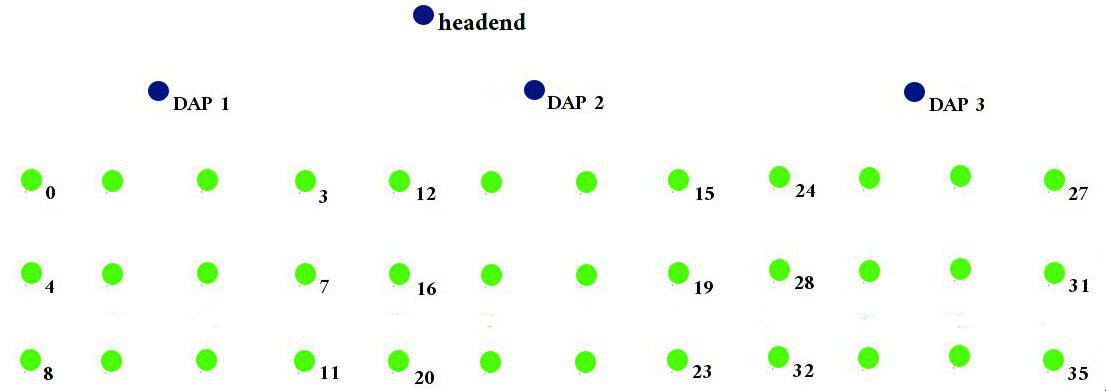
\includegraphics[scale=.23]{IEEE-consolidados/grid36.jpg}
\caption{Scenario used in the simulation.}
\label{mapa}
\end{figure}


\begin  {figure}[hbt]
\begin{minipage}[b]{1\linewidth}
\centering
\subfigure[Packet delivery for all nodes]
{\label{pdf:a}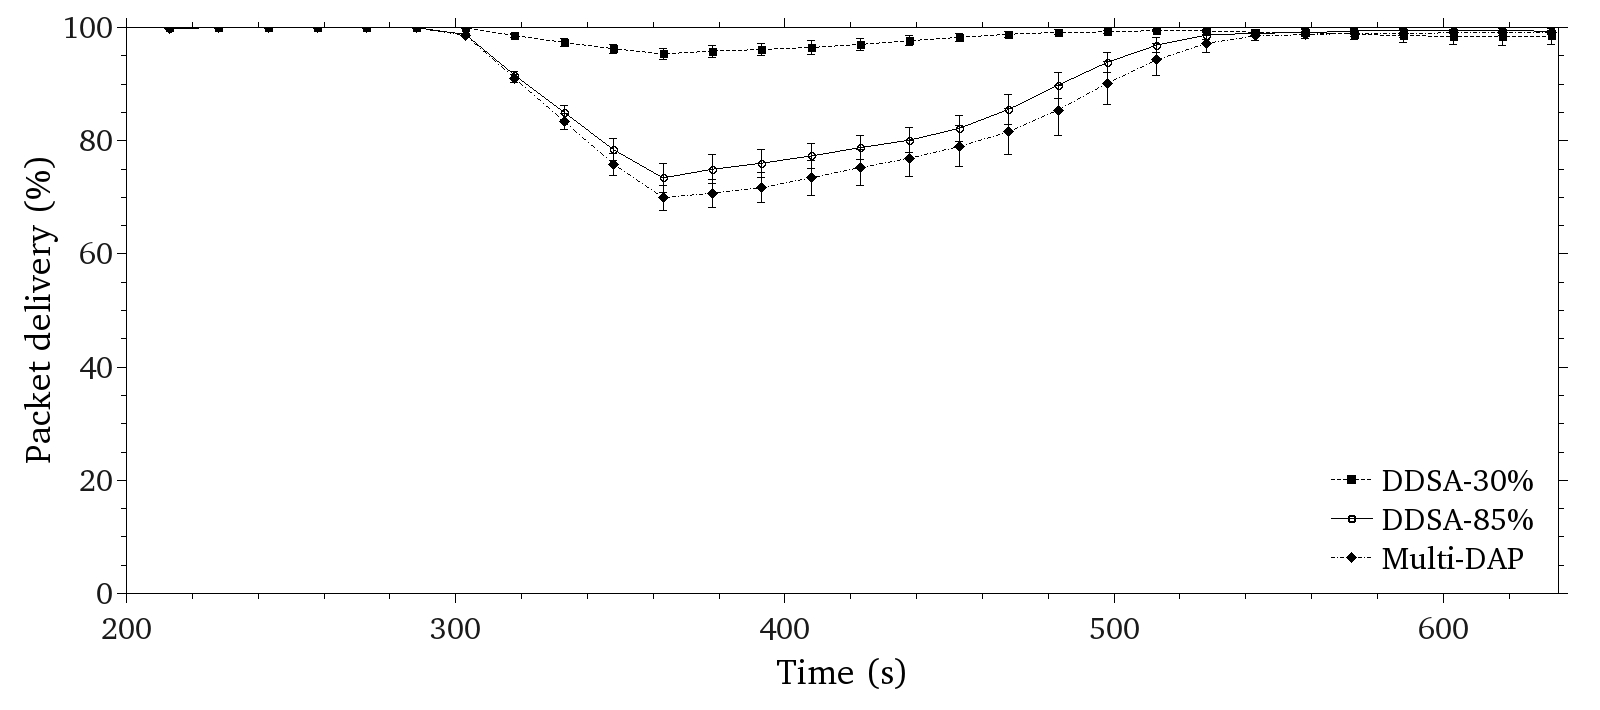
\includegraphics[scale=.21]{IEEE-consolidados/G-pdf-app-desl.jpg}}

\subfigure[Packet delivery for nodes 12-23]
{\label{pdf:b}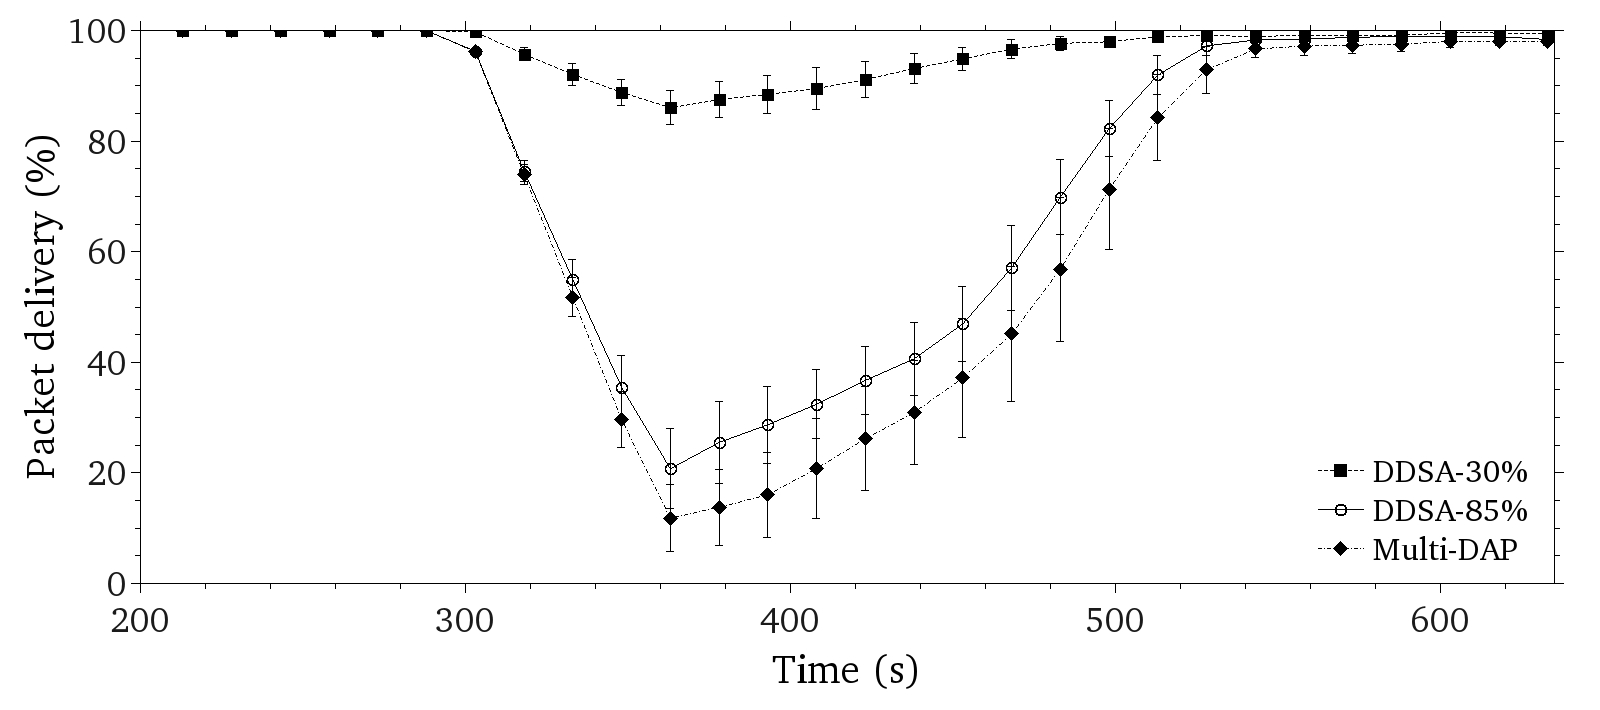
\includegraphics[scale=.21]{IEEE-consolidados/G-pdf-app-centro.jpg}}

\subfigure[Packet delivery for node 16]
{\label{pdf:c}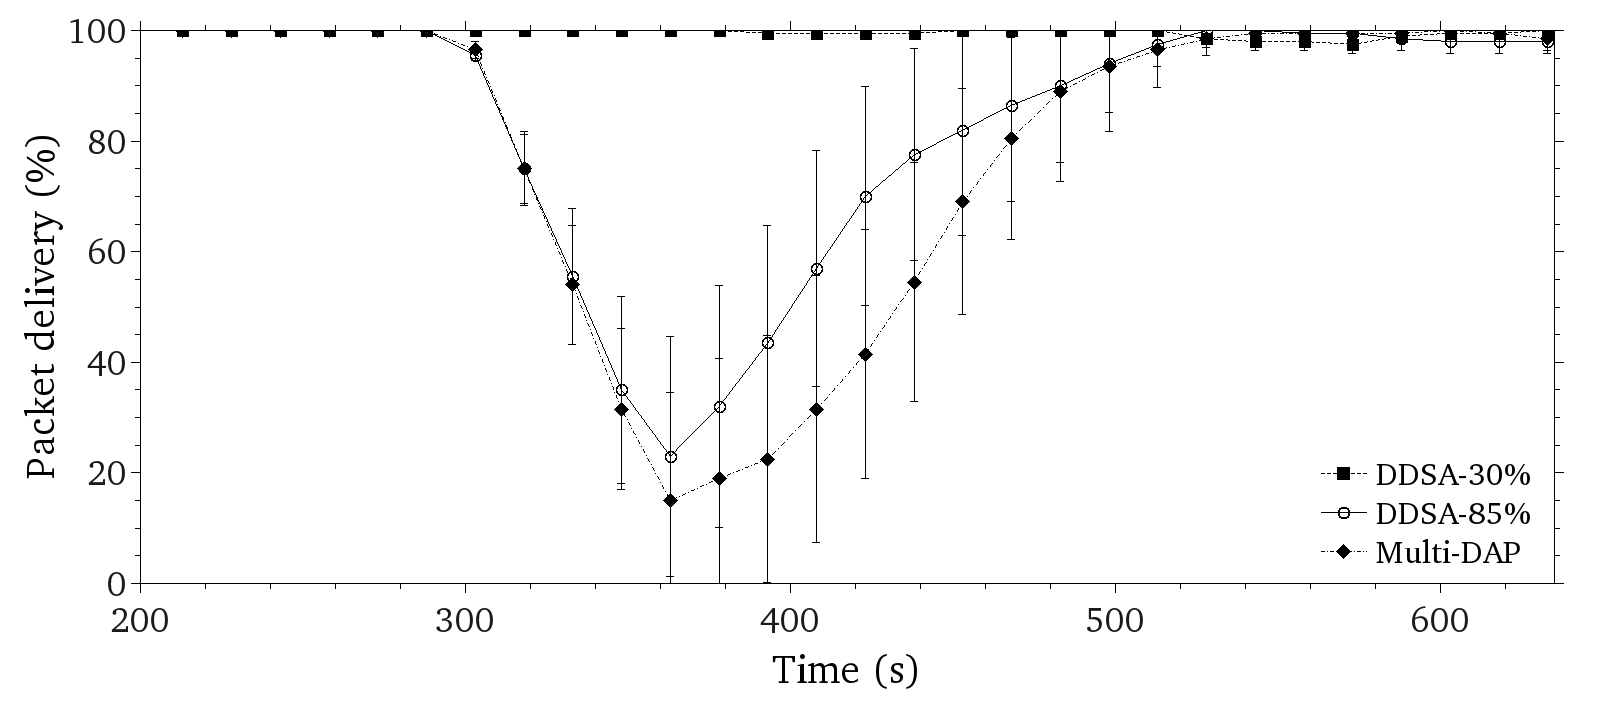
\includegraphics[scale=.21]{IEEE-consolidados/G-pdf-app-16.jpg}}
\end{minipage}
\caption{Packet delivery rates.}
\label{pdf-app}
\end{figure}





\begin{figure*}[ht]
  \centering
  \mbox{
    \subfigure[DDSA-30\%\label{DDSA-30}]{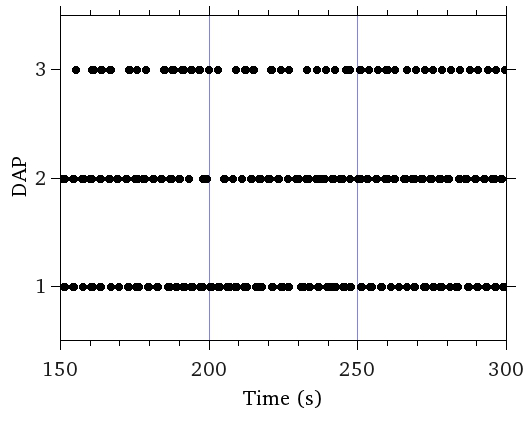
\includegraphics[scale=.31]{IEEE-consolidados/G-troca-gw-ddsa30.jpg}}\quad
    \subfigure[DDSA-85\%\label{DDSA-85}]{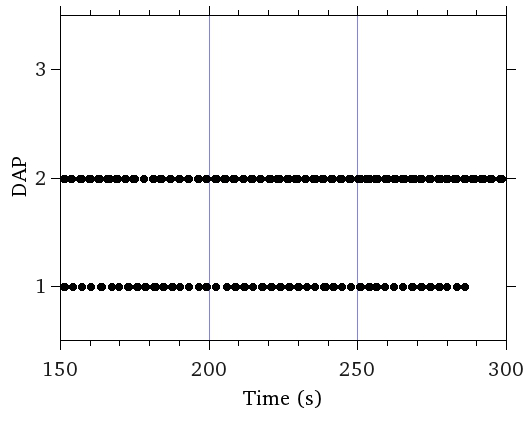
\includegraphics[scale=.31]{IEEE-consolidados/G-troca-gw-ddsa85.jpg}}\quad
    \subfigure[Multi-DAP\label{Multi-DAP}]{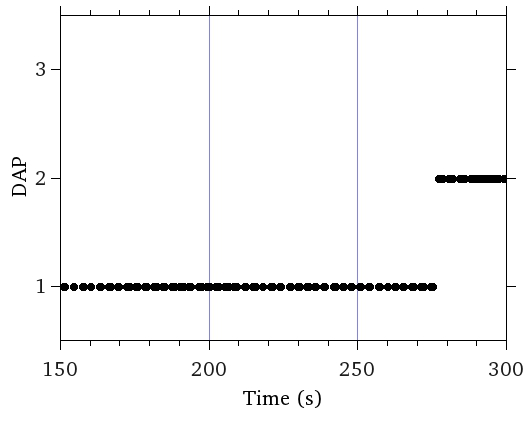
\includegraphics[scale=.31]{IEEE-consolidados/G-troca-gw-multidap.jpg}}
  }
  \caption{DAP choice by node 16 before failure.}
  \label{n16-dap}
\end{figure*}

\begin{figure*}[ht]
  \centering
  \mbox{
    \subfigure[DDSA-30\%\label{DDSA30-2}]{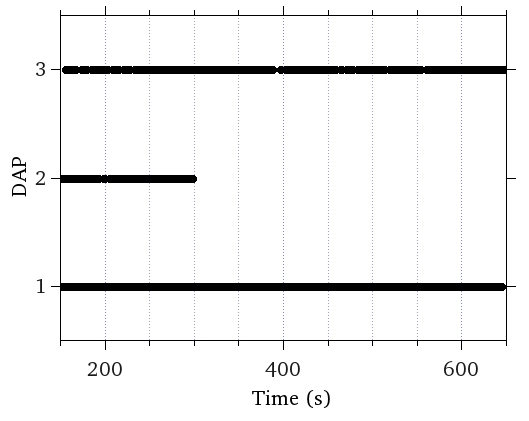
\includegraphics[scale=.31]{IEEE-consolidados/G-troca-gw-ddsa30-2.jpg}}\quad
    \subfigure[DDSA-85\%\label{DDSA85-2}]{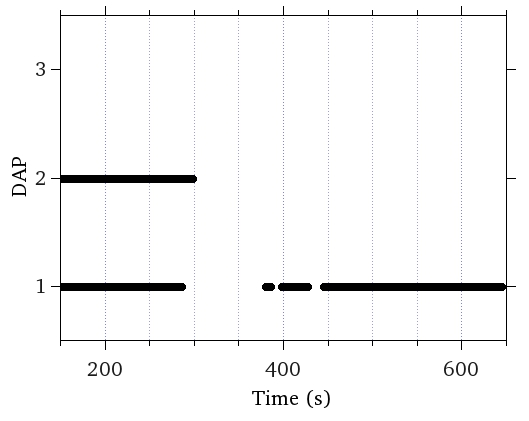
\includegraphics[scale=.31]{IEEE-consolidados/G-troca-gw-ddsa85-2.jpg}}\quad
    \subfigure[Multi-DAP\label{MultiDAP-2}]{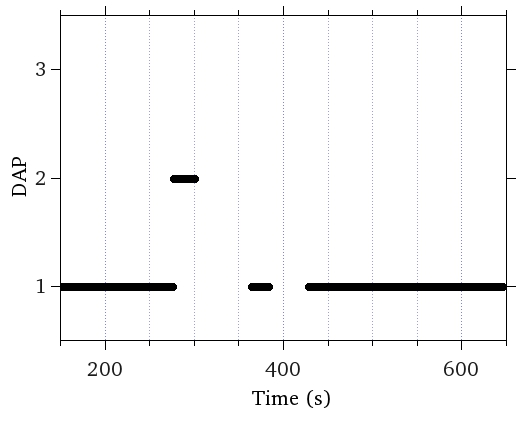
\includegraphics[scale=.31]{IEEE-consolidados/G-troca-gw-multidap-2.jpg}}
  }
  \caption{DAP choice by node 16.}
  \label{n16-dap2}
\end{figure*}


 

\begin  {figure}[ht]
\begin{minipage}[b]{1\linewidth}
\centering
\subfigure[DDSA-30\%]
{\label{dist:a}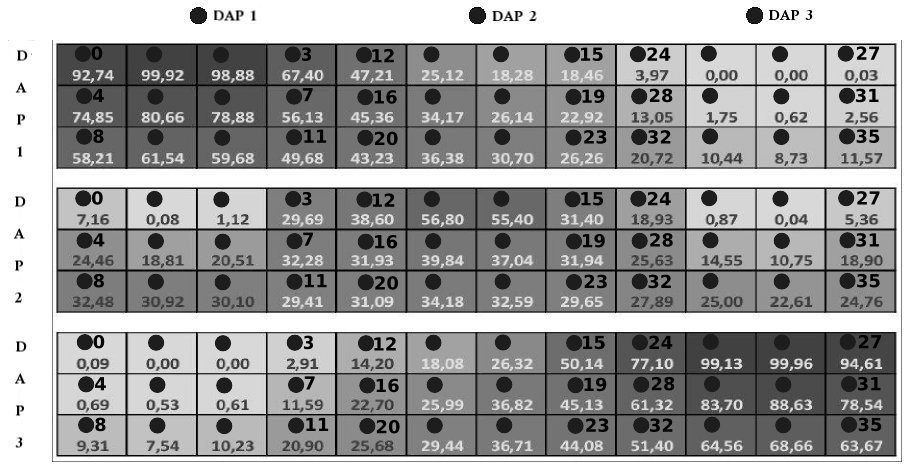
\includegraphics[scale=.28]{IEEE-consolidados/dist-30.jpg}}

\subfigure[DDSA-85\%]
{\label{dist:b}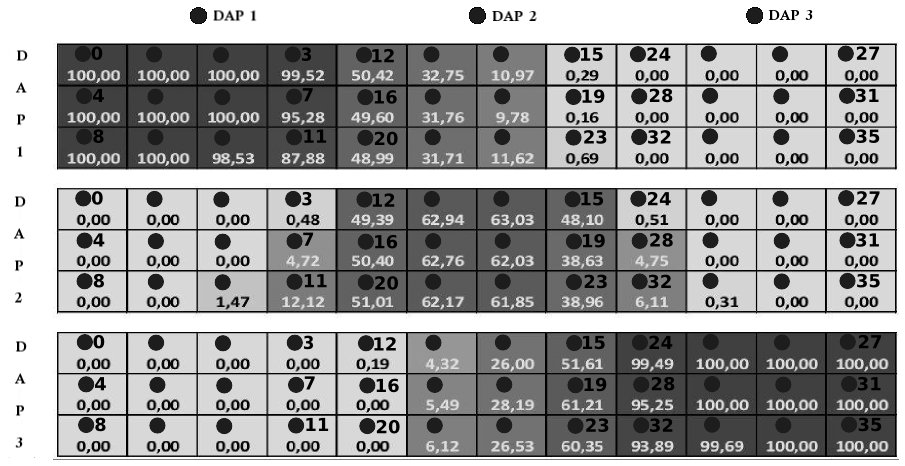
\includegraphics[scale=.28]{IEEE-consolidados/dist-85.jpg}}

\subfigure[Multi-DAP]
{\label{dist:c}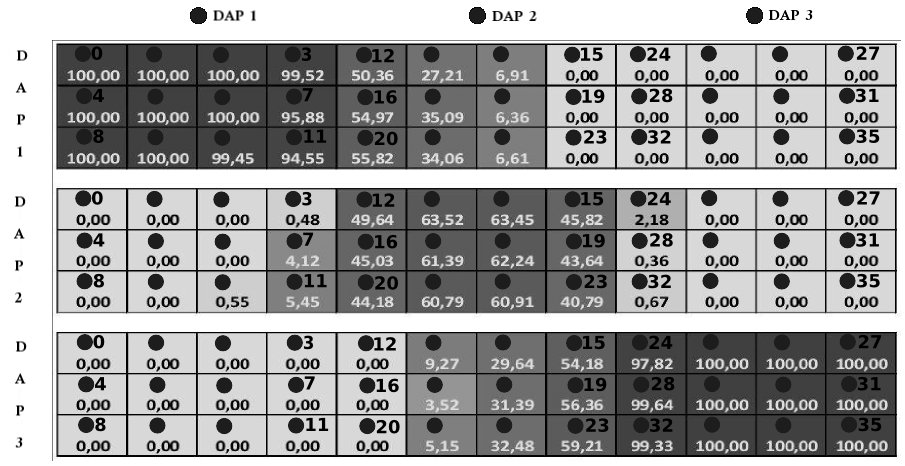
\includegraphics[scale=.28]{IEEE-consolidados/dist-multi.jpg}}
\end{minipage}
\caption{Percentage of DAP usage by each node.}
\label{dist-app}
\end{figure}

The used simulation topology is composed of 36 nodes arranged in a grid and 3 DAPs (Fig.~\ref{mapa}). To simulate the exchange of information between meters and DAPs in a typical application of AMI, a Constant Bit Rate (CBR) UDP traffic is used with fixed packet size of 400B \cite{Plan2011} at the rate of 20 packets per minute. Each node sends 25 flows of data in a synchronized way for every three seconds forcing network congestion. The UDP is an unreliable transport protocol, but has some advantages such low latency. To make it more reliable we used an application protocol over UDP that implements its own transport service suitable for AMI traffic \cite{RFC6272}. The packet delivery rate was calculated for the application layer. We compute as failure in delivery packet if none of the flows in a round are received by any of the DAPs. The exchange of information starts at time 150 seconds and at 300 seconds  DAP 2 fails. A total of 10 simulations were performed with a duration of 650 seconds each and in charts the confidence interval is 95\%.

The DDSA was implemented in ns-2 simulator using OLSR \cite{clausen2003optimized} as the routing protocol. MARA \cite{6051505} was employed as the routing metric and rate adaptation. In assessing the results the following solutions were evaluated:

\begin{itemize}
  \item[(1)] DDSA with $\alpha$ = 0.3 referred to DDSA-30\%;
  \item[(2)] DDSA with $\alpha$ = 0.85 referred to DDSA-85\%; and
  \item[(3)] the mechanism of \cite{Silva2010} for dynamic gateway selection that chooses the best DAP  according to routing metric at the time of sending the data packet. We refer to this as Multi-DAP.
\end{itemize}


\subsection{Simulation Results}



Figure~\ref{pdf:a} shows the packet delivery rate for all nodes as a function of time, considering the latest 60 seconds. It is noticeable that the performance of DDSA-30\% is better than the others proposals after the occurrence of the DAP failure. At time 363 seconds DDSA-30\% has about 95\% of packet delivery rate, while DDSA-85\% has 73\% and Multi-DAP has only 69\% of packets delivery. 
This happens because DDSA-30\%, mainly in central region of the network (nodes 12 to 23), is less affected by the failure of the DAP 2. This can be noticed in Figure~\ref{pdf:b} that shows, at time of 363 seconds, about 86\% of packet delivery rate while DDSA-85\% and Multi-DAP have only 20,7\% and 11,8\%, respectively. This shows that the design choice of distributing packets among DAPs makes it more robust and resilient than others when a failure occurs. 
Figure~\ref{pdf:c}  analyzes the behavior of the packet delivery rate for one node. Node 16 was chosen because it is located geographically between two DAPs. Notice that with DDSA-30\%, when DAP 2 fails, the reduction in the rate was not as sharp as for the other proposals, becoming 77\% and 85\% better than DDSA-85\% and Multi-DAP, respectively, at time 363 seconds. 



To understand how the behavior of DDSA differs from the behavior of Multi-DAP in terms of DAP selection, in Figure~\ref{n16-dap} we show the choices of node 16 using the three proposals during the simulations with a single seed for the period prior to the DAP failure. 
As seen, the choice of $\alpha$ affects the behavior in choosing the DAP. Notice how the lower $\alpha$ (Fig.~\ref{DDSA-30}) causes the farthest DAP (DAP 3) to be eventually chosen.
The higher $\alpha$ (Fig.~\ref{DDSA-85}) makes choices alternating between DAP 1 and DAP 2 that are closest and have better metrics, excluding DAP 3 for having a quality that is too low.
The Multi-DAP (Fig.~\ref{Multi-DAP}) rarely makes exchanges between DAPs, having only used one different DAP in the last 25 seconds of the graph.


Figure~\ref{n16-dap2} shows the same information of Figure~\ref{n16-dap}, but extends the view to the whole period of simulation. 
After the occurrence of the DAP failure at time 300 seconds it is verified that the packets from nodes 16 are not received by any DAP for a long time in the simulations with DDSA-85\% and Multi-DAP.
For DDSA-85\%(Fig.~\ref{DDSA85-2}), the gap to deliver new packets lasted 64 seconds. For Multi-DAP (Fig.~\ref{MultiDAP-2}), the gap lasted 81 seconds. This happens because before the failure they were sending packets only to DAP 2. Note that for DDSA-30\% (Fig.~\ref{DDSA30-2}), there is no noticeable gap because node 16 already balances the load among all DAP.


To check if this behavior is shared by other nodes, we gathered the information shown in Figure~\ref{dist-app}. We show the DAP choices for all nodes using intensities of grayscale to represent the percentages of DAP choices by nodes. Higher values are represented by darker gray and lower values by lighter gray. Each matrix represents the percentages of choices for one DAP and each element is a representation of the  nodes position.  Notice that DDSA-30\% (Fig.~\ref{dist:a}) has a much more balanced DAP selection than the other proposals, as shown by the elements with intermediate gray. For nodes in the central region of the network with DDSA-30\% the lowest value is 14,2\%. For DDSA-85\% (Fig.~\ref{dist:b}) and Multi-DAP (Fig.~\ref{dist:c}) six nodes (nodes 12, 15, 16, 19, 20, 23) ​​do not choose  DAP 1 or DAP 2. Except by nodes 13 and 14, in DDSA-30\% all values in the central region are below 40\% for DAP 2. For DDSA-85\%, all values are above 38\% and for Multi-DAP they are above 40\%. This demonstrates that DDSA-30\% distributes more evenly the packets among DAPs  in central region of network, improving the resilience against DAP failures.


\begin{figure*}[htb]
  \centering
  \label{intv-dap}{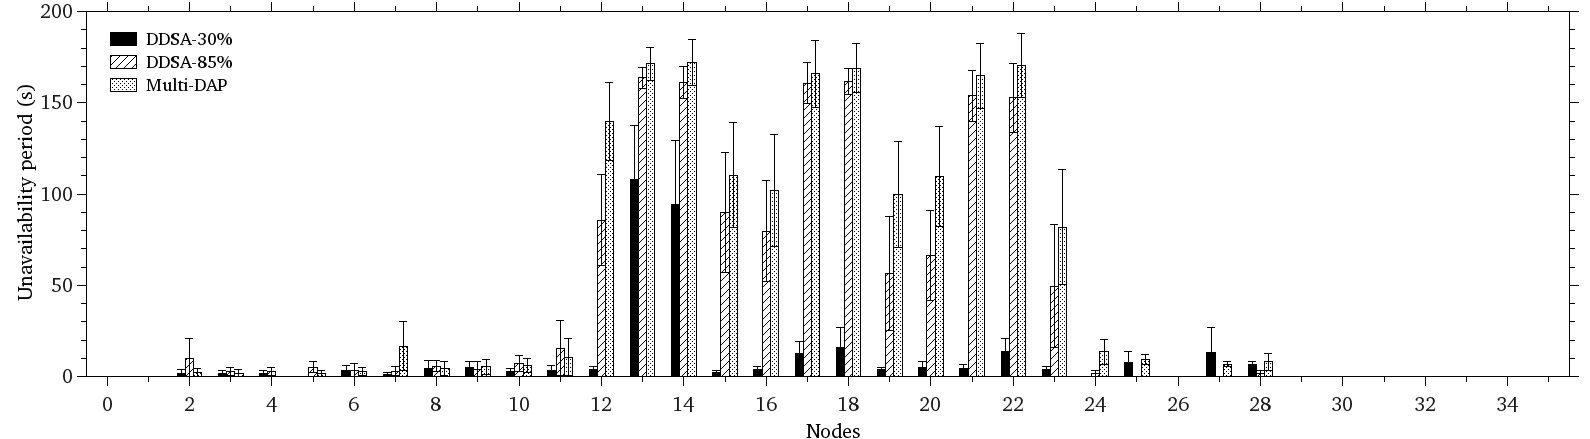
\includegraphics[scale=.31]{IEEE-consolidados/G-wo-rcv-pkt.jpg}} 
  \caption{Unavailability Period.}
  \label{sum-intv}
\end{figure*}


Figure~\ref{sum-intv} shows the unavailability period $\tau$ for each node with respect to the headend,\textit{ i.e.}, the sum of the periods during which each node could not reach the headend through any DAP. 
 It is noticed that the long gap to deliver new packets, as seen for node 16, is repeated for other nodes in the central region of the network. For DDSA-85\% and Multi-DAP these nodes suffered long $\tau$ to deliver packets to any DAP, while DDSA-30\% sustained lower $\tau$. 
Nodes 13 and 14 are the closest ones to the failed DAP 2, thus suffering more influence of this failure, because its path cost is much better compared to the other DAP. Except for these nodes, the average unavailability period $\tau_{avg}$ for the DDSA-30\% is 8,7 seconds and the maximum unavailability period $\tau_{max}$ is 94 seconds. For DDSA-85\%, $\tau_{avg}$ is 37,4 seconds and $\tau_{max}$ is 161,6 seconds, and for Multi-DAP $\tau_{avg}$ is 46,3 seconds and $\tau_{max}$ is 171,3 seconds. 



%\begin{figure}[ht]
%  \centering
%  \label{intv-dap}{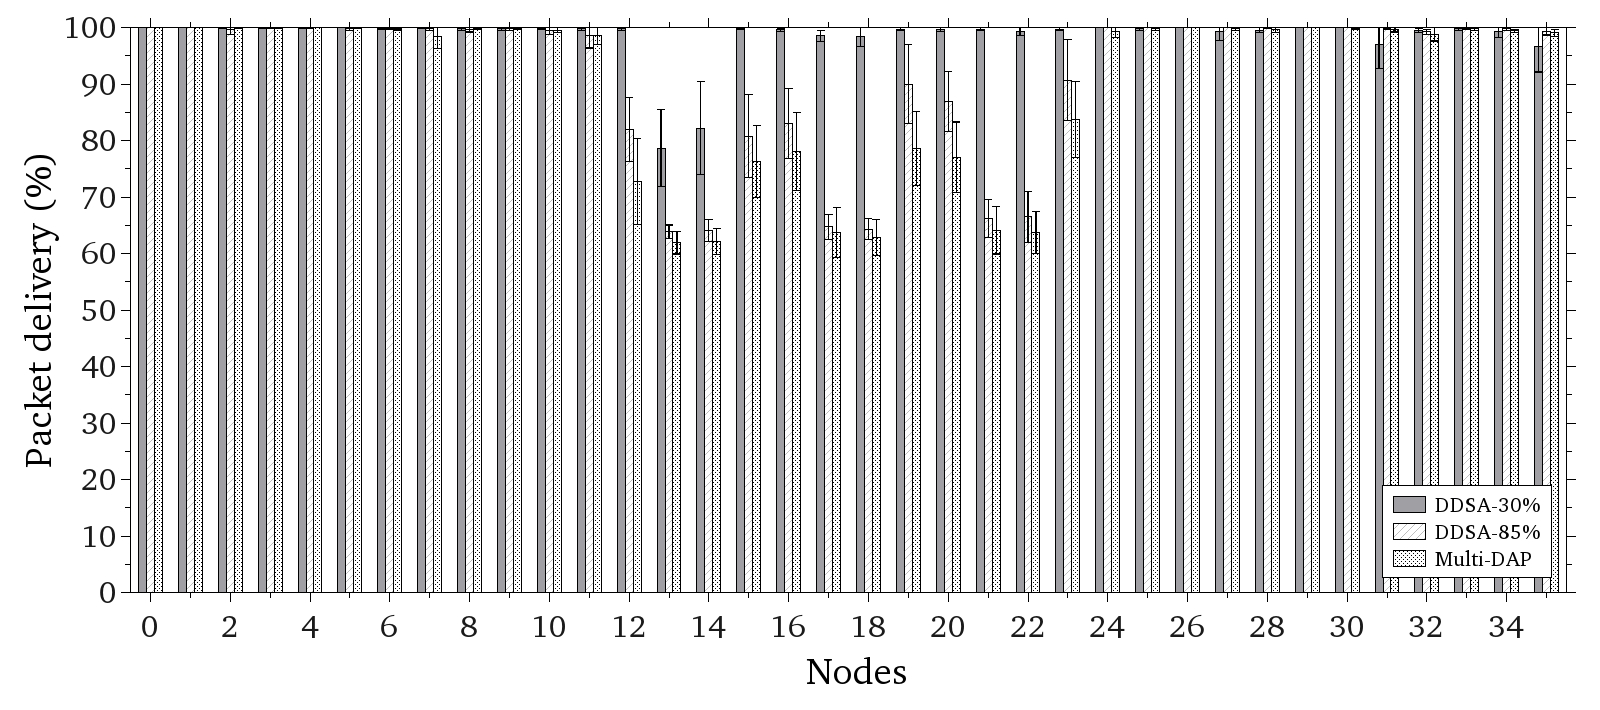
\includegraphics[scale=.21]{IEEE-consolidados/G-no-pdf-app.jpg}} 
%  \caption{Packet delivery}
%  \label{pdf-node}
%\end{figure}


\begin{figure*}[ht]
  \centering
  \mbox{
    {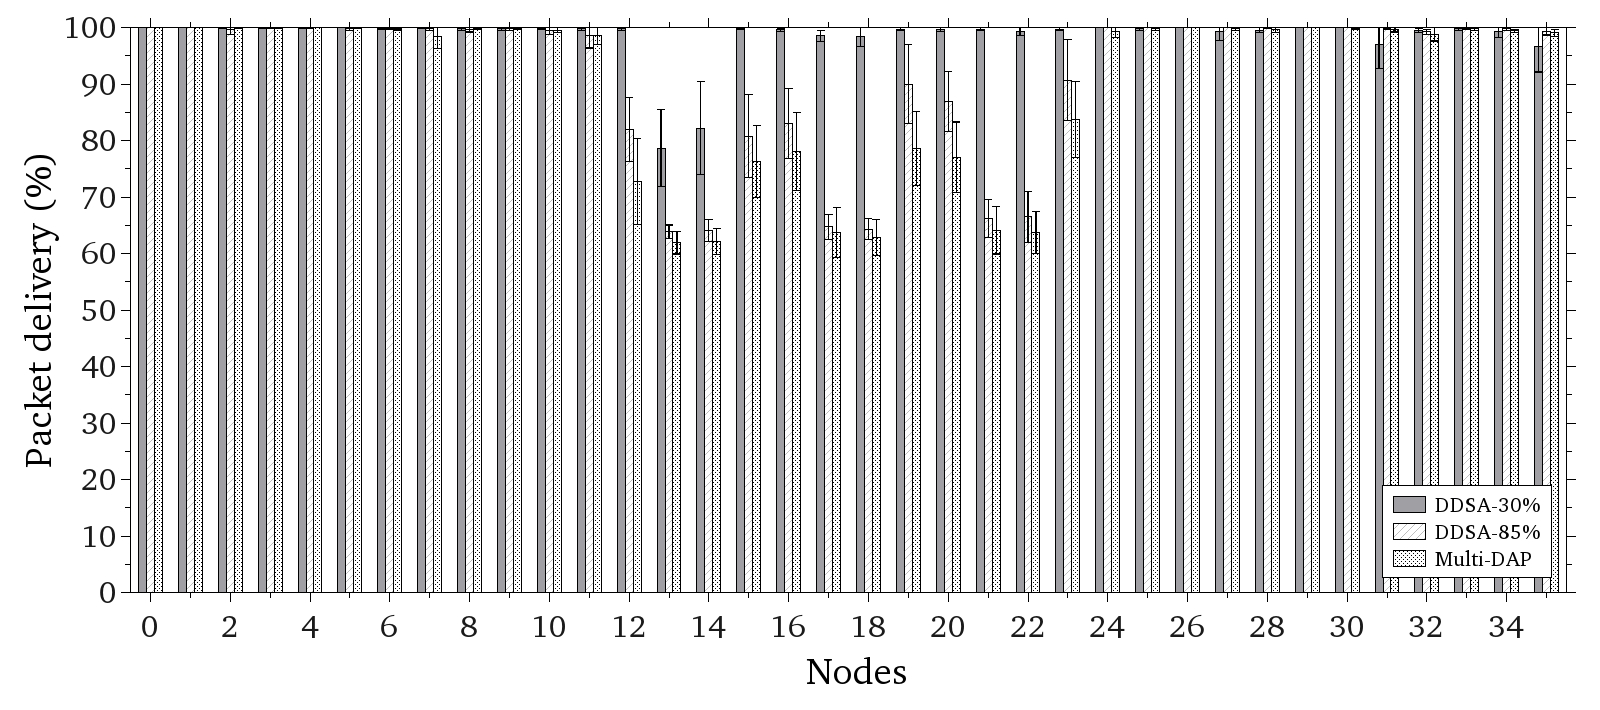
\includegraphics[scale=.31]{IEEE-consolidados/G-no-pdf-app.jpg}}
  }
  \caption{Packet delivery rate for each node.}
  \label{pdf-node}
\end{figure*}


Finally, Figure~\ref{pdf-node} shows the packet delivery rate for all nodes considering all simulation time. It is observed that the central region of the network is the most affected by the failure of the DAP. For these nodes, DDSA-30\% is the less affected by the fault with a performance above DDSA-85 \% and Multi-DAP, for which most of nodes in the central region showed a low packet delivery rates.

\section{Conclusion}

This work presented DDSA, a dynamic DAP selection algorithm to increase the reliability and resilience of AMI applications through the use of multiple DAPs in WMN networks. In this kind of network, the DAP has an important role in exchanging information between the meter and the headend because all traffic flows through it. A failure in a DAP inhibits the exchange of information on the AMI network, so alternative routes through other DAPs should be used after failure to sustain communication between meters and headend.

The results obtained showed that the DDSA increased the resilience of routing protocol even suffering with DAP failure evidenced by lower loss in performance. The results also showed the importance of the choice of the $\alpha$ parameter that influences the routing behavior. Lower values favor resilience, because DDSA distributes packets among more DAPs.


For future work we intend to do a deeper analysis of the impact of the $\alpha$ parameter to observe the behavior of DDSA and find values that bring more resilience or improving performance in routing. 
We also intend to study the use of dynamic adaptation of the $\alpha$ parameter and to analyze other metrics to improve the performance and resilience in a region with failure.


% if have a single appendix:
%\appendix[Proof of the Zonklar Equations]
% or
%\appendix  % for no appendix heading
% do not use \section anymore after \appendix, only \section*
% is possibly needed

% use appendices with more than one appendix
% then use \section to start each appendix
% you must declare a \section before using any
% \subsection or using \label (\appendices by itself
% starts a section numbered zero.)
%



% use section* for acknowledgement
\section*{Acknowledgment}


This work is supported in part by CNPq, CAPES, FAPERJ, TBE/ANEEL and CELESC/ANEEL.


% Can use something like this to put references on a page
% by themselves when using endfloat and the captionsoff option.
\ifCLASSOPTIONcaptionsoff
  \newpage
\fi



% trigger a \newpage just before the given reference
% number - used to balance the columns on the last page
% adjust value as needed - may need to be readjusted if
% the document is modified later
%\IEEEtriggeratref{8}
% The "triggered" command can be changed if desired:
%\IEEEtriggercmd{\enlargethispage{-5in}}

% references section

% can use a bibliography generated by BibTeX as a .bbl file
% BibTeX documentation can be easily obtained at:
% http://www.ctan.org/tex-archive/biblio/bibtex/contrib/doc/
% The IEEEtran BibTeX style support page is at:
% http://www.michaelshell.org/tex/ieeetran/bibtex/
%\bibliographystyle{IEEEtran}
% argument is your BibTeX string definitions and bibliography database(s)
%\bibliography{IEEEabrv,../bib/paper}
%
% <OR> manually copy in the resultant .bbl file
% set second argument of \begin to the number of references
% (used to reserve space for the reference number labels box)
\bibliographystyle{IEEEtran}
\bibliography{./sbc-template}

% biography section
% 
% If you have an EPS/PDF photo (graphicx package needed) extra braces are
% needed around the contents of the optional argument to biography to prevent
% the LaTeX parser from getting confused when it sees the complicated
% \includegraphics command within an optional argument. (You could create
% your own custom macro containing the \includegraphics command to make things
% simpler here.)
%\begin{biography}[{\includegraphics[width=1in,height=1.25in,clip,keepaspectratio]{mshell}}]{Michael Shell}
% or if you just want to reserve a space for a photo:

\begin{IEEEbiography}[{\includegraphics[width=1in,height=1.25in,clip,keepaspectratio]{picture}}]{John Doe}
\blindtext
\end{IEEEbiography}

% You can push biographies down or up by placing
% a \vfill before or after them. The appropriate
% use of \vfill depends on what kind of text is
% on the last page and whether or not the columns
% are being equalized.

%\vfill

% Can be used to pull up biographies so that the bottom of the last one
% is flush with the other column.
%\enlargethispage{-5in}




% that's all folks
\end{document}



